\chapter{Conflicting goals in software development}
\begin{parlist}
	\item All four goals cannot be achieved equally at their maximum capabilities, rather it should be a balanced distribution of them. If quality was taken as example; it would be impossible to reach a great level of quality whilst keeping the costs low and the elapsed time to completion  very short. Also having a great scope for the software and achieving great quality would in any case take a lot of time to be fully complete.\cite{Sommerville:1986aa}
	\item A piece of software that served the purpose of providing programming classes and exercises for third-world countries would have priority in keeping low the maintenance costs and the  running costs. \\ A piece of software with the intention of computing molecules for the covid-19 vaccine has like main goal to be developed in the shortest time possible in order decrease the level of mortality of the virus. \\ A software with the goal of evaluating x-ray scans for potential cancer masses, has to be of the greatest quality possible to provide a near to perfect diagnosis of the patient.\\ An University Management software has to provide multiple functions: a class management system, a class scheduling system, a calendar system or also an archive and a catalogue of many courses and exams. So its scope  should be large enough to incorporate all these requirements. \\
	\begin{figure}[hbt]
  \centering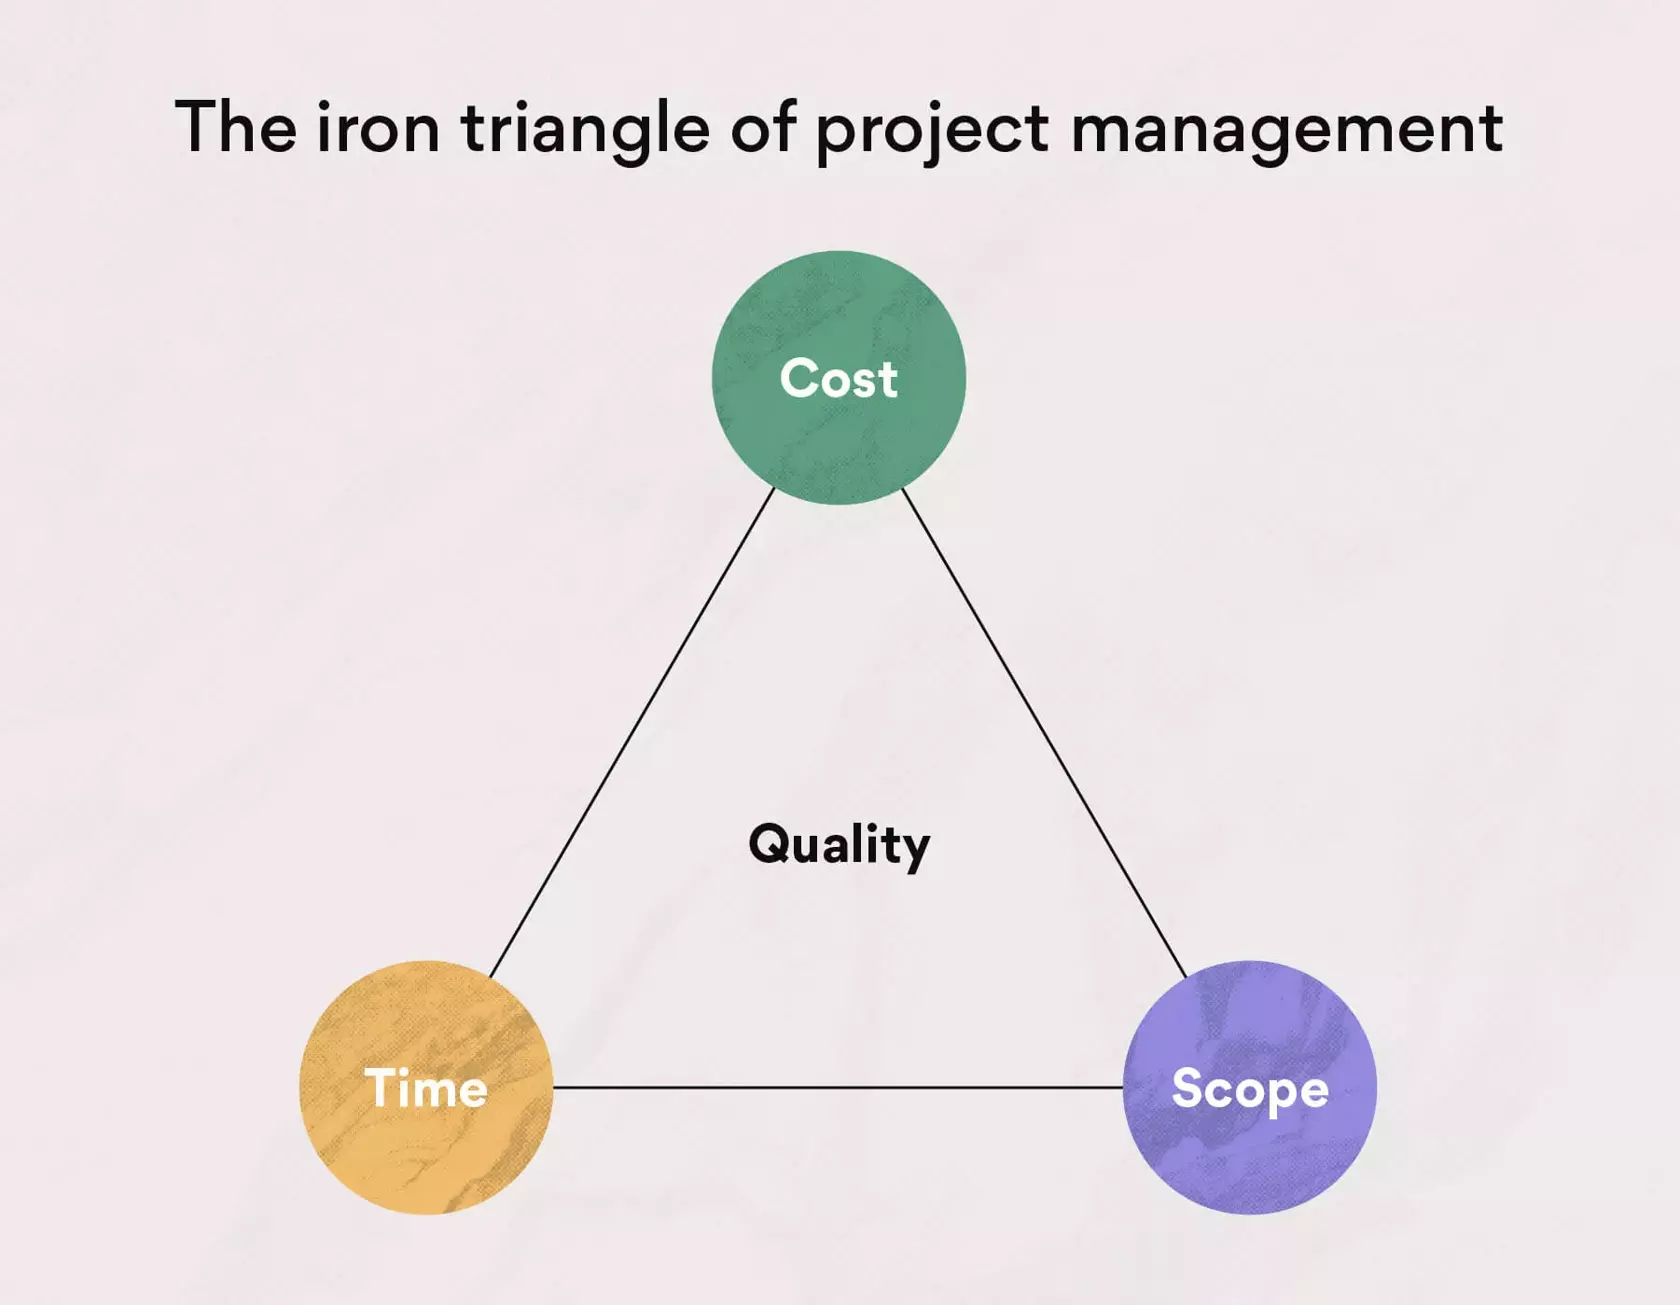
\includegraphics[width=0.5\textwidth]{Immagini/pm.png}
  \caption{Triangle Constraint}
  \label{fig1}
\end{figure}

	\item It's possible to combine the most important goals for software development with a constraint triangle as seen in the figure \ref{fig1}\cite{asana_2022}. At the vertexes there are: Cost,Time and Scope with the central goal being the quality of the software. The principle behind this triangle is that vertexes of the triangle must always be developed equally together. Scope is directly proportional to Time and Cost, since increasing the scope necessary means increasing the cost and the time of the project. Time and Cost, on the other hand, are inversely proportional since, cutting one down means increasing the other and vice versa. The tight correlation between these 3 key aspects makes it so that altering one goal cause a corresponding change in the others.
	\item As discussed earlier Time and Cost in a project are inversely proportional. Cutting budget on production and human resources means more time spent developing the amount of work that could have been done by many more people working on the same project. \\ Assuming that a software developer would need 1 year development time for a software with defined scope and quality, one would like to understand how long it takes 2/5/150 developers to execute the same project. Making a note about the relation between cost and time-it's safe to say that the scenario in which there is only one developer working on the project, it's the one with the least cost. Following the principles stated above, the scenario with 150 developers is the one with the highest cost.\\ Continuing with the subject of \# of developer vs time spent developing; often times increasing the amount of people working on the same project could come with some trade offs. More people working means also more potential mistakes and more time spent coordinating the various parts working together; thus plateauing the benefits from the increased workforce. More people working on the same project also means to define various standards to be able to understand fluently each others work. This can also very frequently happen with even just 2 people working on the same project. \cite{alma990004140290402883}
\end{parlist}
	